\documentclass[runningheads]{llncs}

\usepackage{amsmath}
\usepackage{booktabs}
\usepackage{graphicx}
\usepackage{url}

\setlength{\textfloatsep}{8pt plus 2pt minus 2pt}
\setlength{\floatsep}{6pt plus 2pt minus 2pt}
\setlength{\intextsep}{6pt plus 2pt minus 2pt}
\emergencystretch=2em

\begin{document}

\title{Fact-Constrained Multimodal Retrieval for Orthodontic Report Generation from Intraoral Scans and Photographs}
\titlerunning{Fact-Constrained Multimodal Orthodontic Report Retrieval}

\author{Yan Sun}
\authorrunning{Yan Sun}
\institute{Independent participant, ODIN 2026\\
\email{sunyan@cmu.edu.cn}}

\maketitle

\begin{abstract}
We present a fact-constrained multimodal retrieval system for ODIN 2026 Task 2 (Bite2Text), which generates an orthodontic diagnostic report from paired intraoral scans and photographs. Rather than decoding free text, the method retrieves a clinically written report and constrains its selection with structured evidence. Paired meshes are standardized with IOS-Normalizer; a Point Transformer V3 (PTv3) encoder predicts 12 orthodontic attributes; and a five-view ResNet18 supplies complementary evidence for eight cross-validated attributes. A 3,720-dimensional geometric descriptor retrieves 50 candidates, which are ranked by geometric similarity, PTv3 agreement, and photographic soft agreement. Conservative midline correction, unsupported-fact filtering, and contradiction-risk reranking are applied only under cross-validated gates. On strict five-fold out-of-fold evaluation of 867 labeled cases, the final method obtained BLEU-4 0.2684 and METEOR 0.4700. The final container operates without network access and processes one case in approximately 27--40 seconds.

\keywords{Orthodontics \and Intraoral scan \and Multimodal retrieval \and Report generation \and Point Transformer}
\end{abstract}

\section{Introduction}

ODIN 2026 Bite2Text requires generation of a diagnostic report from upper and lower intraoral scans (IOS) and intraoral photographs \cite{odin2026}. The output must be fluent, but factual consistency is particularly important: RadFact-F1 contributes 80\% of the final score, while BLEU-4 and METEOR each contribute 10\%.

Direct generation can introduce unsupported tooth-specific findings, whereas a fixed template driven by a small label set is constrained but incomplete. We therefore formulate Bite2Text as fact-constrained retrieval. The system selects a complete report from the training collection using standardized 3D geometry, PTv3-derived attributes, and photographic evidence. Narrow corrections are enabled only when supported by patient-separated out-of-fold (OOF) validation.

Our contributions are: (1) deterministic paired-scan normalization and quality control; (2) a 12-head PTv3 model and complementary five-view photographic model; (3) multimodal clinical-report retrieval; (4) precision-oriented filtering and contradiction-aware reranking; and (5) an offline Docker implementation compatible with the official interfaces.

\begin{figure}[t]
  \centering
  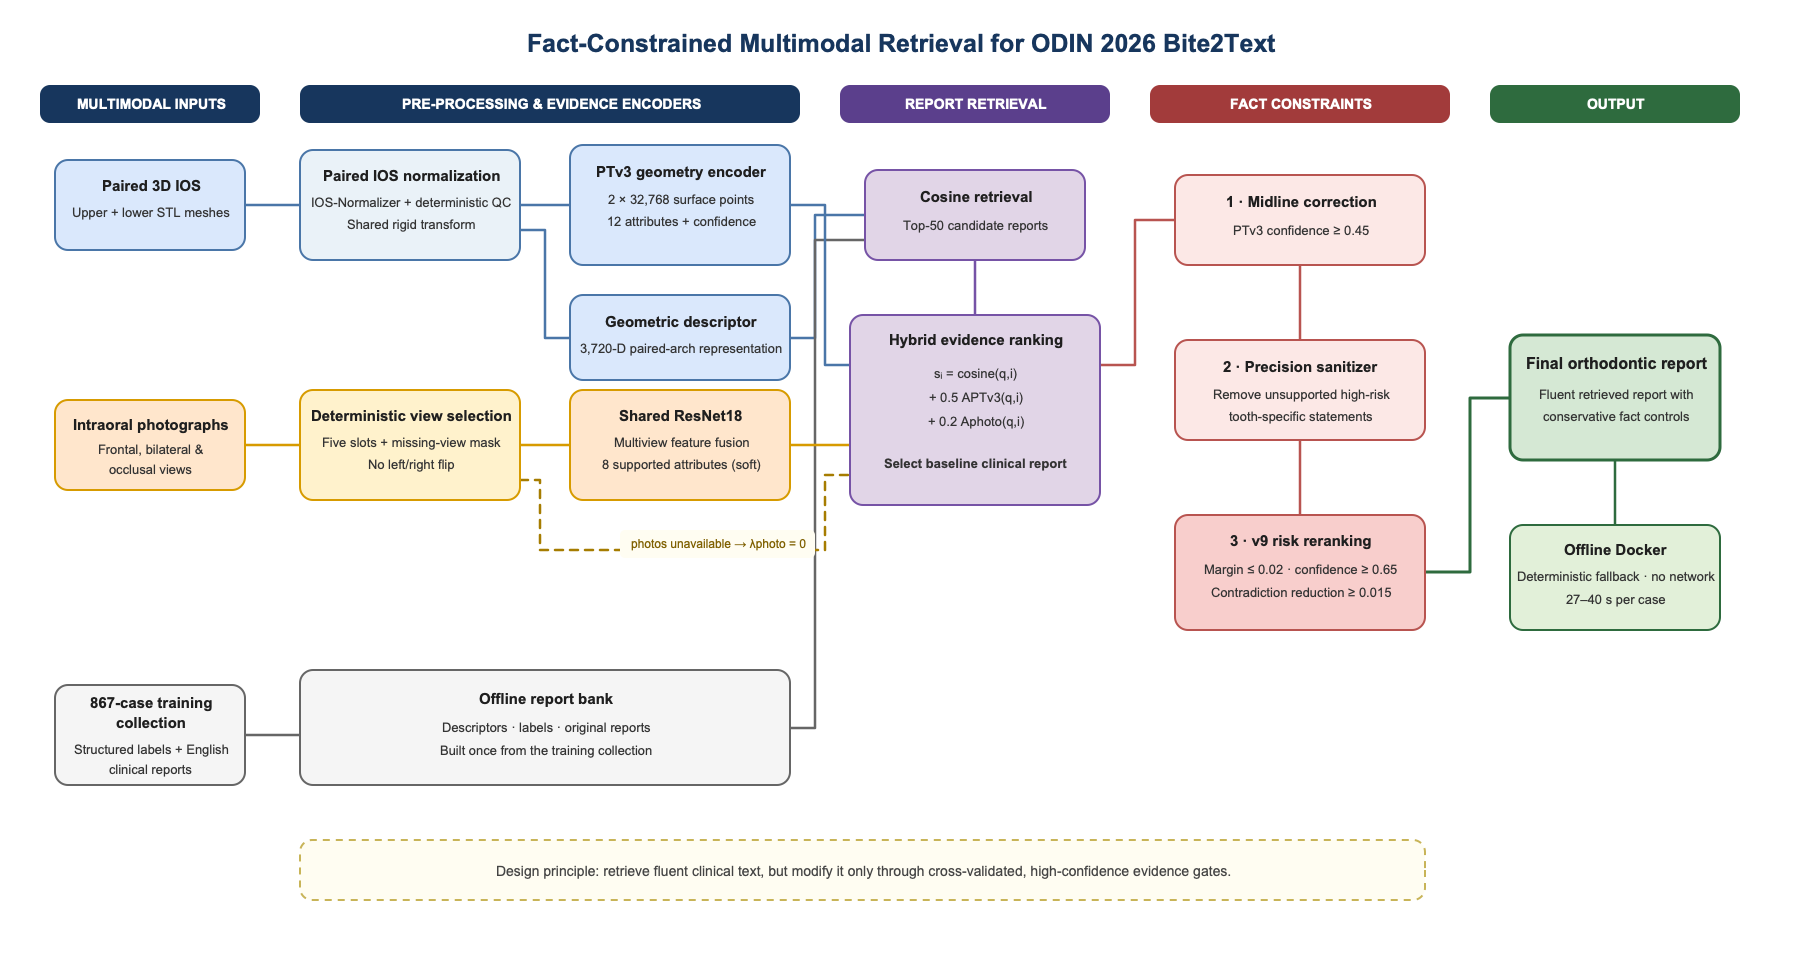
\includegraphics[width=\textwidth]{../figures/ODIN2026_Task2_Technical_Route.png}
  \caption{Fact-constrained multimodal retrieval pipeline. Missing or unreadable photographs trigger a deterministic geometry-only fallback.}
  \label{fig:pipeline}
\end{figure}

\section{Data and Pre-processing}

The supervised development set contained 867 patients: 190 from Bits2Bites \cite{bits2bites} and 677 from the challenge release. Each case could contain paired meshes, photographs, an English report, and 12 structured attributes: bilateral molar and canine relation, overjet, vertical and midline relation, crossbite, upper and lower crowding, and the curves of Spee and Wilson.

The IOS audit found 993 non-empty upper/lower pairs; one additional case had empty meshes. Raw orientation was heterogeneous: 437 arches were primarily aligned with the XZ plane and 556 with the XY plane. IOS-Normalizer \cite{iosnormalizer} estimated a paired rigid orientation, followed by conservative case-level corrections that preserved the upper/lower relationship. All 993 pairs were normalized, and 992 passed automatic orientation quality control. The remaining case contained a large scan base and was not part of the supervised cohort. Proper rotations were retained, with maximum orthogonality error $8.04\times10^{-7}$ and coordinate residual below $7.5\times10^{-6}$.

The photographic audit contained 5,213 images from 997 folders; one image was unreadable. There were 867 cases with exactly five images, 124 with more than five, and six with fewer than five, yielding 11 missing view slots. A ResNet18 \cite{resnet} classified frontal, lateral, and occlusal views with patient-separated accuracy 0.9329 and macro-F1 0.9359. Global assignment selected one frontal, two lateral, and two occlusal views while discouraging near duplicates. Missing slots were masked.

\section{Method}

\subsection{Structured 3D and Photographic Evidence}

We adapted PT-v3m1 \cite{ptv3} from Bits2Bites to 12 class-weighted heads. The model uses nine input channels and encoder widths 16, 32, 48, 64, and 128. Training froze the encoder for 10 epochs, followed by joint fine-tuning. Five folds selected joint-training epochs 17, 59, 47, 38, and 48; their median, 47, was fixed before unified training on all 867 labeled cases. AdamW used learning rate $10^{-4}$, weight decay 0.01, batch size 8, grid size 0.01, and cosine annealing. Mean fold-specific macro-F1 was $0.4586\pm0.0100$.

The photographic model uses a shared ImageNet-pretrained ResNet18, learned view-slot embeddings, mean/max/flatten fusion, and 12 heads. Horizontal flipping was disabled to preserve clinical left/right semantics. Photo-only OOF macro-F1 was 0.3845, so photographs did not replace 3D decisions. Only eight supported attributes were retained: bilateral canine relation, overjet, vertical relation, midline relation, bilateral crowding, and Curve of Wilson. A coefficient of 0.2 was selected independently in all outer folds. Fusion raised structured OOF macro-F1 from 0.4544 to 0.4651.

\subsection{Report Retrieval and Fact Controls}

Each query is represented by a 3,720-dimensional descriptor of the normalized paired arches. Cosine similarity retrieves the 50 nearest training cases. Candidate $i$ is scored as
\begin{equation}
s_i=\operatorname{cosine}(q,i)+0.5A_{\mathrm{PTv3}}(q,i)+0.2A_{\mathrm{photo}}(q,i),
\end{equation}
where $A_{\mathrm{PTv3}}$ is reliability-weighted hard-label agreement and $A_{\mathrm{photo}}$ is photographic soft agreement. Reliability weights are OOF macro-F1 values; missing labels contribute zero.

Three narrow controls are then applied. First, only the dental-midline sentence may be corrected, and only when PTv3 confidence is at least 0.45. Second, a precision sanitizer targets anomalously detailed reports and removes unsupported tooth-specific claims about restorations, caries, eruption, attachments, and demineralization; it changed 7/867 OOF reports. Third, v9 considers a replacement candidate only within a retrieval-score margin of 0.02 and when the original conflicts with a PTv3 prediction of confidence at least 0.65. Its adjusted score is
\begin{equation}
s_i^{\mathrm{risk}}=s_i-0.005N_{\mathrm{unsupported}}(i)-0.5R_{\mathrm{contradiction}}(i).
\end{equation}
Replacement additionally requires contradiction-risk improvement of at least 0.015 and no increase in unsupported sentences. Otherwise, the output is byte-identical to v8a.2. This gate changed 8/867 OOF reports.

\section{Experiments and Results}

All choices used patient-separated five-fold validation with fold sizes 172, 173, 173, 174, and 175. A validation query could retrieve reports only from the other four folds. BLEU-4 and METEOR used the challenge evaluator. RadFact-Lite \cite{radfact} with GLM-5.2 \cite{glm} was used only as a paired local proxy; it was never called during challenge inference.

\begin{table}[t]
\centering
\caption{Strict OOF component ablation over 867 cases.}
\label{tab:ablation}
\small
\begin{tabular}{lccc}
\toprule
Method & BLEU-4 & METEOR & Mean \\
\midrule
Geometry retrieval & 0.2513 & 0.4523 & 0.3518 \\
$+$ PTv3 agreement (v5) & 0.2646 & 0.4660 & 0.3653 \\
$+$ photo agreement (v6) & 0.2653 & 0.4667 & 0.3660 \\
$+$ midline correction (v7) & 0.2677 & 0.4694 & 0.3685 \\
$+$ precision sanitizer (v8a.2) & 0.2672 & 0.4691 & 0.3681 \\
$+$ risk reranking (v9) & \textbf{0.2684} & \textbf{0.4700} & \textbf{0.3692} \\
\bottomrule
\end{tabular}
\end{table}

Table~\ref{tab:ablation} shows progressive improvement. Direct verbalization of the 12 attributes was substantially weaker (BLEU-4 0.1735, METEOR 0.3472) than PTv3-constrained retrieval. Photographic evidence produced a small consistent gain without overriding PTv3; midline correction gave the largest post-retrieval text improvement.

The sanitizer improved proxy RadFact-Lite F1 from 0.2190 to 0.3308 across its seven affected cases, with seven wins and no losses. Across the eight cases changed by the final risk gate, F1 rose from 0.2634 to 0.3680; final precision and recall were 0.3700 and 0.3659. Seven cases improved and one decreased. These subset results are model-selection evidence, not official hidden-test scores.

\begin{table}[t]
\centering
\caption{Organizer-reported hidden-test metrics over 50 cases as of 18 August 2026.}
\label{tab:hidden}
\small
\begin{tabular}{lcccc}
\toprule
Submission & BLEU-4 & METEOR & RadFact-F1 & Final score \\
\midrule
Earlier v7 & 0.2145 & 0.4569 & 0.3660 & 0.3600 \\
Final v9 & \textbf{0.2151} & 0.4512 & not released & not released \\
\bottomrule
\end{tabular}
\end{table}

The v9 evaluation succeeded on 50 hidden cases, with BLEU-4 $0.2151\pm0.1164$ and METEOR $0.4512\pm0.1207$. Its official RadFact-F1 had not yet been released when this report was prepared. Consequently, the temporary leaderboard based on available text metrics is not the final challenge ranking.

\section{Deployment, Reproducibility, and Limitations}

The amd64 Docker image accepts the official upper IOS, lower IOS, and photograph interfaces and writes one JSON report. Missing or unreadable photographs trigger the 3D-only path. Eleven unit tests and three end-to-end cases passed under network isolation, a 16~GB host-memory limit, and one GPU. Runtime was 27--40 seconds per case.

\begin{table}[h]
\centering
\caption{Exact final-submission identifiers.}
\label{tab:identifiers}
\footnotesize
\begin{tabular}{@{}ll@{}}
\toprule
Item & Identifier \\
\midrule
Display name & \texttt{Bite2text Report} \\
URL slug & \url{qwen3-vl-photo-orthodontic-report} \\
Image version & \url{174a2e7b-25dd-40a0-b282-83a27b9b5aab} \\
Model version & \url{41720d11-653a-4d48-8ce6-d3d575bd0fd7} \\
Submission & \url{e5588ed6-a164-4561-83f1-7b541a62fd3a} \\
Evaluation & \url{3fac9821-fc34-45c4-bb1b-df4b912e28f7} \\
Source commit & \url{0d0d83e1a962f361bc3b70e4d36ae129d338708b} \\
\bottomrule
\end{tabular}
\end{table}

Code and assembly instructions are available at \url{https://github.com/Shayne-Pro/ODIN2026-Bite2Text}.

The method retrieves a report written for another patient. Structured reranking reduces incompatible occlusal statements, but source reports may retain patient-specific details not supported by the query. The sanitizer cannot prove entailment for every sentence, and the photographic model remains less accurate than PTv3. The local RadFact proxy differs from the official evaluator. Outputs are for research evaluation only and require expert review before any clinical use.

\section{Conclusion}

We combined standardized IOS geometry, PTv3 structured prediction, multiview photographic evidence, and complete-report retrieval. Conservative, cross-validated fact controls improved strict OOF text metrics and targeted factuality while preserving deterministic offline deployment. Future work should replace sentence-level heuristics with calibrated multimodal entailment trained on dental evidence.

\begin{thebibliography}{7}

\bibitem{odin2026}
ODIN 2026 Grand Challenge: Task 2 -- Bite2Text. \url{https://odin2026.grand-challenge.org/} (accessed 18 August 2026)

\bibitem{bits2bites}
AImageLab-zip: Bits2Bites. Commit \texttt{8c3c685}. \url{https://github.com/AImageLab-zip/Bits2Bites}

\bibitem{iosnormalizer}
AImageLab-zip: IOS-Normalizer. Commit \texttt{ecebe110}. \url{https://github.com/AImageLab-zip/IOS-Normalizer}

\bibitem{ptv3}
Wu, X., Jiang, L., Wang, P.-S., Liu, Z., Liu, X., Qiao, Y., Ouyang, W., He, T., Zhao, H.: Point Transformer V3: Simpler, Faster, Stronger. In: CVPR, pp. 4840--4851 (2024)

\bibitem{resnet}
He, K., Zhang, X., Ren, S., Sun, J.: Deep Residual Learning for Image Recognition. In: CVPR, pp. 770--778 (2016)

\bibitem{radfact}
AImageLab-zip: RadFact-Lite. Commit \texttt{053f680}. \url{https://github.com/AImageLab-zip/radfact_lite}

\bibitem{glm}
Zhipu AI: GLM-5.2 API. \url{https://open.bigmodel.cn/} (accessed 18 August 2026)

\end{thebibliography}

\end{document}
